\documentclass[11pt,a4paper]{article}
\usepackage[T1]{fontenc}
\usepackage[margin=1in]{geometry}
\usepackage{amsmath,amssymb,mathtools}
\usepackage{booktabs}
\usepackage{graphicx}
\usepackage{xcolor}
\usepackage[colorlinks=true,linkcolor=blue!60!black,citecolor=blue!60!black,urlcolor=blue!60!black]{hyperref}
\usepackage{microtype}
\usepackage{xurl}
\setlength{\emergencystretch}{3em}
\usepackage{enumitem}
\usepackage[most]{tcolorbox}
\newtcolorbox{keybox}[1][]{colback=blue!3,colframe=blue!45!black,boxrule=0.5pt,left=4pt,right=4pt,top=3pt,bottom=3pt,#1}
\newtcolorbox{failbox}[1][]{colback=red!3,colframe=red!45!black,boxrule=0.5pt,left=4pt,right=4pt,top=3pt,bottom=3pt,#1}
\hypersetup{pdftitle={Gated exciton fluids III},pdfauthor={Xavier Callens},pdfsubject={Matrix-free Newton-Krylov solver; classical node arrangements with the Fenris-CMRR engine}}

\begin{document}
\begin{center}
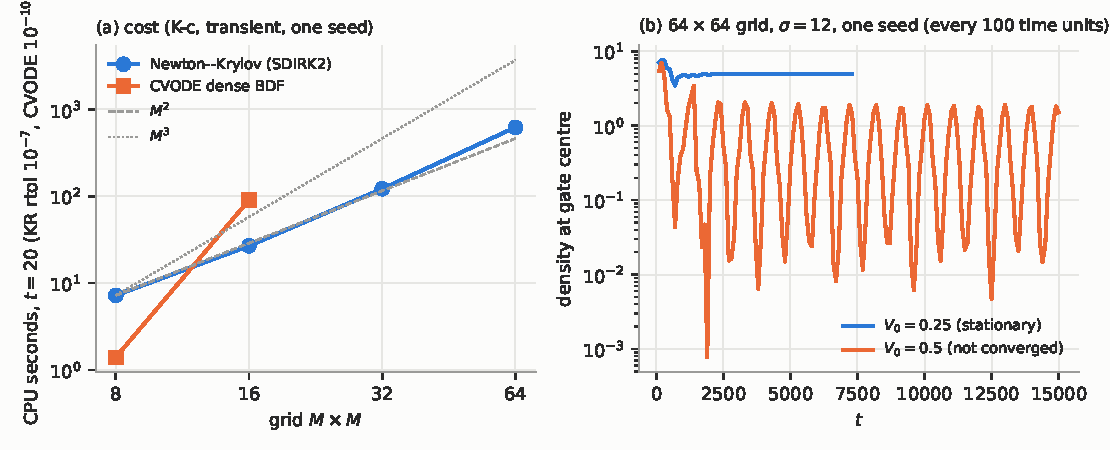
\includegraphics[width=0.97\textwidth]{figs_companion3/fig_krylov.pdf}\\[4pt]
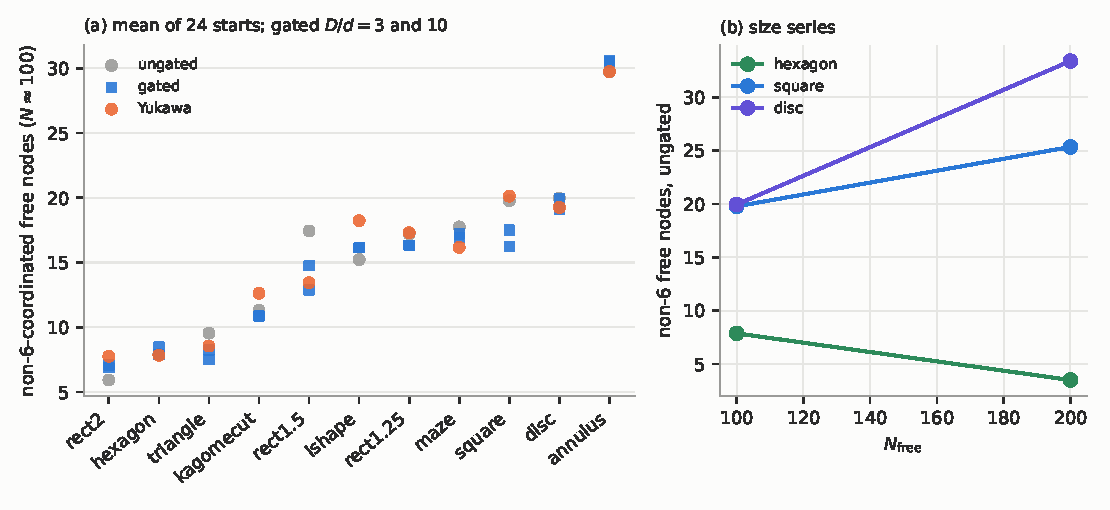
\includegraphics[width=0.97\textwidth]{figs_companion3/fig_fenris.pdf}
\end{center}
\vspace{-0.6em}
\begin{center}
{\Large\textbf{Gated exciton fluids III:}\\[2pt]
\large a matrix-free Newton--Krylov solver and a $64\times64$ case it does not converge,\\ and a classical node-arrangement study of shaped containers with the Fenris-CMRR engine}\\[8pt]
Xavier Callens\\ {\small SocrateAI Research \quad\url{https://github.com/xaviercallens/SocrateAI-Scientific-QuantumFluids}}\\[2pt]
{\small October 2026}
\end{center}
\vspace{-0.4em}

\begin{abstract}\small\noindent
This third paper reports the two work packages that were still running when the second one~\cite{CallensII} was deposited; both are
pre-registered, both ended with a failed or partly failed gate, and both were re-checked by an independent hostile verifier (a separate
AI instance; its notes are committed under \url{docs/designs/EXCITON_FLUID_VERIFIER_NOTES_*.md}).
\textbf{(1)}~A matrix-free implicit solver (two-stage L-stable SDIRK2, GMRES, a Fourier-diagonal block preconditioner, analytic
Jacobian--vector products) for the driven-dissipative exciton model reproduces the dense-CVODE records and the independent reviewer's
digits, is second order in time, and has a CPU cost per transient time unit growing like $M^{2.15}$ between $8\times8$ and $64\times64$
grids (7\,s to 621\,s). For one $t=20$ transient of one seed it is slower than dense CVODE at $8\times8$ and faster at $16\times16$; the cost exponent also mixes
grid and box scaling. The registered $64\times64$ gate
(a stationary state at gate amplitude $V_0=0.5$) is \textbf{not met}: the run does not converge and shows a persistent pulsation of
period about 970 at three resolutions; whether that is physical was not tested independently. The planted-bug gate on the preconditioner
was passed only in a regime where it could not fail, and a second regime test failed for two of six variants.
\textbf{(2)}~A classical relaxation study with the author's Fenris-CMRR engine and the gated kernel in eleven container shapes: the
pre-registered design (wall nodes at the mean spacing, uniform random starts) did not confine the free nodes and was replaced by a
denser wall and random-sequential-addition starts. With that wall model, the number of non-sixfold-coordinated free nodes depends
strongly on the container shape (from about 6 to about 30 at $N\approx100$); the kernel changes it much less at the extremes but not
negligibly in mid-range shapes, and the search statistics are thin. It is a classical design target, not an exciton prediction. Written by an AI system; not refereed.
\end{abstract}

\section{Scope and status}

\begin{keybox}
Papers~I~\cite{CallensI} and~II~\cite{CallensII} are the context. The lattice theorem used upstream~\cite{OpenAI2026} is unrefereed and
AI-generated. Nothing here compares with experimental data. Both packages carry a pre-registration committed before their first
trajectory. \textbf{Amendments and changed gates.} The Krylov amendments A1--A6 were committed before the runs they announce (checked by
the verifier from commit times). For Fenris, A1--A3 were; A4 (random-sequential-addition starts, which defines the production design) was
committed together with the production results and was written after four test cases with the new start, and A5 likewise. Gate criteria
were changed during the work: Fenris A1 rewrote the a4 criterion after it failed (a harness fault), A2.5 added a floor to a1 after it
failed, and A2 set the CVODE tolerance to $10^{-2}$ (L-f then shows energies independent of it to $\le2.9\times10^{-9}$); the Krylov
stopping rule changed twice during the $64\times64$ run (A3, A4: a CPU cap, then a hand stop at $t=15000$, 7.5\% of the registered horizon);
K-d$'$ was added because the original K-d could not fail. Verifier verdicts: Krylov \emph{no blocking item}; Fenris \emph{accept with fixes}.
\end{keybox}

Numbers are read from committed files (named in Section~\ref{sec:repro}) or are the verifiers' recomputations, whose notes are committed; the figures are generated by
\texttt{exploration/exciton/python/companion3\_fig\_krylov.py} and \texttt{companion3\_fig\_fenris.py}. The CVODE timings of the scaling panel are read from \texttt{summary.json}.

\section{A matrix-free Newton--Krylov solver}\label{sec:krylov}

\textbf{Motivation.} Paper~I found dense CVODE (43\,ms per step at 768 unknowns) unusable at $64\times64$, and the ETD integrator of paper~II has no
error control. The pinned rusty-SUNDIALS tree has a GMRES module but no Krylov option in CVODE, so a new implicit stepper was written
outside CVODE (crate \texttt{qf-exciton-kr}). \textbf{Design:} two-stage L-stable SDIRK2 with an embedded first-order error estimate and
adaptive steps; inexact Newton; GMRES(20), right-preconditioned by the Fourier-diagonal kinetic factor combined with the pointwise
$3\times3$ inverse of the reservoir block (so one application costs two FFTs); exact analytic $Jv$. For stationary states a
pseudo-transient mode with frame tracking and a looser tolerance is used (amendment A1).

\begin{center}\small
\begin{tabular}{@{}p{0.09\textwidth}p{0.12\textwidth}p{0.69\textwidth}@{}}
\toprule
gate & outcome & numbers (verifier's recomputation from the raw records) \\ \midrule
K-a1 & pass & $8\times8$, $V_0=0.5$ against the CVODE records at $t=4000$: $|\Delta\omega|=1.0\times10^{-8}$, $|\Delta n_c|=9.7\times10^{-6}$,
full state $1.2\times10^{-6}$ \emph{after phase alignment} (0.94 unaligned: the state rotates); at $t=16000$ ($\mathrm{rtol}=10^{-4}$, A1): $2\times10^{-11}$ and $2.2\times10^{-9}$ \\
K-a2 & pass & $16\times16$, $t=100$: relative $L^2$ error $9.1\times10^{-6}$, $9.2\times10^{-7}$, $1.2\times10^{-7}$ for rtol $10^{-6},10^{-7},10^{-8}$
(monotone); CPU 64, 189, 436\,s against CVODE 549\,s (the $\Delta n_c$ gate is met at $10^{-7}$ and not at $10^{-6}$) \\
K-a3 & pass 6/6 & against the independent reviewer's printed digits only (2--4 digits): a rounding-level agreement \\
K-b & pass & errors $1.06\times10^{-3},\ldots,4.81\times10^{-6}$; ratios $3.56,3.89,3.98,4.00$: \textbf{second order}; started on the slaved
manifold, so it tests no stiff transient \\
K-c & pass & median CPU for $t=20$, rtol $10^{-7}$, 3 repeats: $7.22,\ 26.8,\ 122,\ 621$\,s at $M=8,16,32,64$; exponent 2.15 (8--64), local slopes 1.9, 2.2, 2.35 \\
K-d1--d4 & pass, weak & badsign needs $1.508\times$ the GMRES iterations (gate 1.5); jac bug gives identical counts and is caught only by a unit test; rhs bug
differs from CVODE by 2.6; all in a regime where the preconditioner cannot matter (A2) \\
K-d$'$ (A2) & \textbf{4 of 6} & block (reference), kin, jac, fd: 1.03--1.05 GMRES per Newton, 50--72\,s; rhs bug caught (shift error 8.4); badsign: 10.6 (1142\,s, converged but shift error $2.0\times10^{-7}$ against a $10^{-7}$ gate: \textbf{fail}); none: 23.0, not converged at the
$t=2\times10^5$ cap (residual $4\times10^{-6}$, 1415\,s) \\
K-e0,e1,e3 & pass & stationary states to residual $<10^{-7}$ in 7--2100 CPU\,s (the largest is the $64\times64$ R64 run); seed spread $5\times10^{-8}$; rtol $10^{-4}$ vs $10^{-6}$ shift differs by $6\times10^{-9}$;
shifts for the $L=16$ box on $M=16,32,64$ grids $0.0766598, 0.0767908, 0.0768237$ (differences $1.3\times10^{-4}$ then $3.3\times10^{-5}$: second-order convergence) \\
K-e2 & \textbf{not met} & $64\times64$, $\sigma=12$, $V_0=0.5$: residual $4\times10^{-3}$--$2\times10^{-2}$ for $t>2000$; stopped by hand at
$t=15000$ (7761\,CPU s, as registered in A4) \\
\bottomrule
\end{tabular}
\end{center}

\noindent{\footnotesize\textbf{Cover figure, top.} (a) Cost against grid size: the Krylov solver (median of three repeats) grows like $M^{2.15}$; dense CVODE (rtol $10^{-10}$) is
faster at $8\times8$ and 3.4$\times$ slower at $16\times16$ (no CVODE run was made at 32 or 64). (b) Density at the gate centre sampled every 100 time
units on the $64\times64$ grid: $V_0=0.25$ converges, $V_0=0.5$ does not (peak heights are sampling-aliased).}

\textbf{What the cost result does and does not say.} The exponent 2.15 is for a transient of 20 time units, three repeats of one
seed, at machine load 4--8 on 8 cores, and its local slope is still rising (per-step exponents 1.9, 2.5, 2.3); in this series the box
$L=M$ and $\sigma\propto M$ grow with the grid, so the number of unknowns grows like $M^{2}$ while the solved problem also changes; it
is not a stationary-state cost and not a guarantee for larger grids. Against dense CVODE the solver is \emph{slower} at $8\times8$ (7.2 vs 1.4\,s) and about 3.4--4.9$\times$ faster at $16\times16$
(Krylov rtol $10^{-7}$ against CVODE 90.5\,s at rtol $10^{-10}$ and 132\,s at $10^{-7}$; the latter is longer than at $10^{-10}$, an
unexplained anomaly, with repeats scattering 108--135\,s; one seed, one transient). Against the ETD integrator of paper~II the
stationary-state times at $8\times8$ and $16\times16$ are of the same order; nothing stronger is claimed.

\begin{failbox}
\textbf{The registered $64\times64$ gate was not met.} It was not demonstrated by $t=15000$ of a registered horizon of $2\times10^5$ (hand stop, A4). For $V_0=0.5$ the pseudo-transient solve does not approach a stationary state:
$n_{\rm center}$ oscillates between 0.005 and 2.07 for $t\ge2000$ (and between $8\times10^{-4}$ and 3.4 earlier), $\omega$ between 0.5607 and
0.5745, 14 peaks with period about 969 by $t=15000$. Diagnostics registered afterwards (A3, no gate) show a pulsation at the coarser
grids of the same box: period 956 at $M=16$ and 966 at $M=32$ (each to $t=40000$, about 40 cycles), 969 at $M=64$ (to $t=15000$ only).
The $M=32$ and $M=64$ waveforms agree to an rms of 0.08 in $n_{\rm center}$ for $1000\le t\le15000$ (about 8\% of the signal rms, a
recomputation by the reviewer; no script is committed) despite different noise realisations, which argues against a pure noise artefact;
the $M=16$ waveform is not as close (rms 0.71, maximum 1.77 against 2.14). \emph{What is not established:} no independent integrator
was run at this geometry; the diagnostic at the tighter tolerance stopped at $t=500$, before the first peak, so tolerance
independence is untested; there was no Newton solve of the fixed point and no linear stability analysis; one seed, one $V_0$, one box.
The safe statement is that the solver does not converge at this point and a persistent pulsation of period about 970 appears at rtol
$10^{-4}$. At $V_0=0.25$ the $64\times64$ run converges (residual $2.2\times10^{-9}$ at $t=7300$, shift 0.0447); a run at $V_0=1$ was
abandoned at $t\sim100$ and has no result.
\end{failbox}

\textbf{Finite-size information obtained along the way (measured, no gate).} At fixed $\sigma=3$ the gate-induced shift of the emission
frequency is $0.0767, 0.0151, 0.00354$ for $L=16,32,64$ (log--log slope $-2.2$; ratio to the area average of the gate $0.69, 0.55, 0.51$),
confirming the box-area artefact reported in paper~I. At fixed $\sigma/L$ for $L=8,16,32$ it is $0.0876, 0.0767, 0.0699$: not size
independent (it falls by $12.5\%$, then $8.8\%$). For $V_0=0.25$: $0.0488, 0.0463, 0.0447$ at $L=8,16,64$. At $L=64$, $V_0=0.5$
there is no stationary shift to report.

\textbf{Process notes.} A1--A6 were committed before the runs they announce (verifier); K-d$'$ was added in A2 because the original K-d could not
fail, and the A2 regime test then failed for two variants; the badsign failure (shift error four times the seed spread $5\times10^{-8}$) and the \textquotedblleft none\textquotedblright\ failure
(non-convergence) are both reported as failures of the registered gate.
The summary file \texttt{summary.json} is the only results record (no report was written), and the second diagnostic ran CPU-starved
(about four times).

\section{Fenris-CMRR: classical node arrangements in shaped containers}\label{sec:fenris}

\textbf{What this is.} The relaxation engine of the author's \texttt{rusty-Fenris-CMRR} (v0.1, commit \texttt{6d0df125})~\cite{Fenris} is
extended by a kernel trait (the Yukawa results are unchanged to $4\times10^{-13}$) to relax free nodes against fixed boundary nodes under:
the ungated dipole kernel ($d=0.5$ in units of the mean boundary spacing), the gated kernel for $D/d=3$ and $10$ (from the Bessel
$K_0$ mode sum of the image representation, analytic first and second derivatives), and a Yukawa control. It is \emph{not} a statement
about excitons: the free nodes are classical particles, the wall is a ring of fixed nodes, and the universal-optimality statements of
the upstream theorem concern infinite periodic configurations and say nothing about this bounded problem.

\textbf{Gates.} L-a (kernel against an independent direct image sum: $4.6\times10^{-13}$ absolute; table against series: relative
$U$ $9\times10^{-14}$, $U'$ $7\times10^{-12}$, $U''$ $8\times10^{-10}$; $K_0,K_1$ against scipy $1.5\times10^{-14}$), L-b (engine: a reported 5 of 6 of the original
suite; the failing test fails on the unpatched tree too, so L-b is not a clean pass), L-c (best energy equal to $1.5\times10^{-14}$ relative to an independent solver in 8 of 8 small cases, but
only one inside minimum per case, so it is a weak test), L-d (planted bugs; bug~1 is not caught by gate a2, disclosed), L-e (Euler bookkeeping,
below) and L-f (energies independent of integrator tolerance to $\le2.9\times10^{-9}$) all pass, after harness amendments A1--A5 that
the verifier judged to raise no threshold to hide a kernel failure. The verifier recomputed energies and forces of five stored best states
with its own kernel and wall (agreement $\le10^{-13}$, $\max|F|\sim10^{-10}$, identical coordination counts) and rebuilt the table of
44 production cases (1056 starts, 1031 accepted, 0 escaped, 36 per-shape means, Spearman, medians).

\begin{failbox}
\textbf{The registered design was not usable.} Wall nodes at the mean spacing and uniform random starts: in 12 primary cases only 0--5
of 24 starts stayed inside (23 of 24 escaped in the ungated square). The study was stopped (A3) and rerun with the wall nodes at half
spacing (extra nodes at midpoints) and random-sequential-addition (RSA) starts, with which 0 of 96 escaped in a square test and all 44
production cases ran with 0 escapes. \emph{The cause is not isolated:} amendment A4 itself shows that at half spacing the escapes with uniform starts came from the violent first
part of the flow (starts with close pairs) and that RSA starts cured them; the spacing-1 wall was never rerun with RSA starts. The result is
therefore only ``spacing-1 wall with uniform random starts: 19--24 of 24 escaped; spacing-1 wall with RSA starts: untested''. The saddle
mechanism proposed in A3 is asserted, not tested.
\end{failbox}

\noindent{\footnotesize\textbf{Cover figure, bottom.} (a) Mean number of non-sixfold-coordinated free nodes at $N_{\rm free}\approx100$ for 11 shapes and four kernels (24 RSA starts
each, accepted states only); (b) ungated kernel at $N_{\rm free}=100$ and $200$.}

\textbf{Production results} (one wall model; 44 cases, $N_{\rm free}\approx100$, 24 starts each; 1031 states accepted at force $\le10^{-6}$ with a
positive-definite Hessian, 1054 of 1056 positive-definite, 90 accepted states not strict).
\begin{itemize}[leftmargin=1.2em,itemsep=1pt]
\item \textbf{Shape dominates at the extremes; the kernel matters less, not nothing.} Mean counts (ungated / gated $D/d=3$ / gated $10$ / Yukawa): annulus $29.7/30.5/30.6/29.8$;
disc $20.0/19.1/19.9/19.3$; square $19.8/17.5/16.2/20.1$; maze $17.8/17.2/16.9/16.2$; L-shape $15.2/16.1/16.1/18.2$; kagome-cut hexagon
$11.3/10.9/10.9/12.6$; triangle $9.5/8.2/7.5/8.5$; hexagon $7.9/8.5/7.9/7.8$; $2{:}1$ rectangle $5.9/7.1/6.9/7.8$. Between-shape standard
deviation 6.3 against 0.79 between kernels within a shape; the shape ordering has Spearman correlation 0.88--0.97 across kernels. The kernel
effect is not negligible: in mid-range shapes the spread over kernels reaches 4.5 (the $1.5{:}1$ rectangle ranges from 12.9 to 17.4), as
large as the gaps between neighbouring shapes; no standard errors are available (a mean of 24 starts with a within-shape deviation near
0.8--1 has a standard error near 0.2, but the starts are not independent samples of a stationary distribution); with $\mathrm{ddof}=1$ the
two deviations are 6.6 and 0.91.
\item \textbf{Defects near the wall: not demonstrated as a concentration.} 30--88\% of the non-6 nodes lie within 1.5 spacings of the wall
(maze 88\%, annulus 68\%, square 30--42\%), so for 5 of 11 shapes not even a majority; the mean number at distance $\ge3$ is at most about
3, so for annulus, maze and L-shape the deep region is almost empty. Per free node the defect density in the deep region is 0.88
(hexagon), 1.38 (triangle) and 1.64 (L-shape) relative to the all-node density, so no wall concentration is shown against that null.
\item \textbf{Size.} Ungated, $N_{\rm free}$ from 100 to 200: hexagon $7.9\to3.5$ (mean $|\psi_6|$ $0.84\to0.93$), square $19.8\to25.4$
($0.71\to0.81$), disc $20.0\to33.4$ ($\times1.67$, above the perimeter ratio $\sqrt2$ that the square's $\times1.28$ roughly follows). The
$N=200$ series has 20 starts per case and no error bars; the commensurate/incommensurate statement rests on three shapes and one size ratio.
\item \textbf{Net topological charge is set by the boundary.} $Q=\sum_{\rm free}(6-c)=6\chi+\sum_{\rm wall}(k_b-3)$ holds exactly for
all 1031 accepted states (0 failures); this is an identity for any conforming triangulation, so the gate tests the code, not the physics,
and $k_b$ itself depends on the state (a standard deviation of $Q$ up to 1.3 within a case). Mean $Q$: hexagon $-4$, triangle $-3.5$, disc $-1.6$,
annulus $-4.6$, maze $+5.7$, rectangles about 0.
\item \textbf{Many minima.} The median fraction of starts reaching the best energy (relative $10^{-6}$) is 0.085 (mostly 1/24); the median
number of distinct minima is 18 of 24; triangle (0.41--0.50) and hexagon (0.04--0.38 at $N=100$) are the exceptions. Best energies are local minima,
not global optima.
\item \textbf{Sensitivity.} With the kernel parameters changed ($d=1$, Yukawa $\kappa=3$; square and hexagon, $N\approx100$) the defect counts move by up to $+16\%$ (square, gated $D/d=10$), $-11\%$ (square, Yukawa) and $+11\%$ (hexagon, Yukawa), and
$|\psi_6|$ by up to 0.06; square and hexagon remain far apart.
\end{itemize}

\textbf{Limits.} All numbers describe one wall model (fixed nodes at half spacing, spacing-1 sites for the triangulation, a built-in 7\%
mismatch between the mean node spacing and the ideal-lattice nearest-neighbour distance); no wall-spacing scan was run, and
$30$--$88\%$ of the defects are within 1.5 spacings of that wall. Statistics are over accepted starts only (25 of 1056 dropped, about 2\%). $N=400,600$ were not run. The
comparison with the open-boundary study of paper~II was attempted and is \emph{not} used: the boundary models differ (penalty wall with
particles in a hull against fixed nodes) and the interior definitions give incomparable numbers. The requested results note was not
written separately; the narrative lives in the amendment texts and this paper.

\section{Reading these results for the laboratory protocol}\label{sec:protocol}

Protocol item L6 of paper~I (edges and frustration) remains a \emph{design target}: the Fenris study supports the statement that, for
fixed-node walls of this kind, the container shape sets the defect count more than the kernel does at the extremes, with a visible kernel effect in mid-range shapes. It does not tell an experimentalist where an exciton lattice will break, and the Krylov
result adds a caveat for the driven-dissipative model: at the registered large box the gate-driven state at $V_0=0.5$ was not found stationary,
so a stationary-state reading of L1 at that amplitude is not supported by these runs.

\section{Limitations and reproducibility}\label{sec:repro}

Single seeds and small statistics for several Krylov items; $64\times64$ at two amplitudes only; the pulsation not tested with an
independent integrator; the Fenris wall model is one choice; the upstream lattice theorem is unrefereed. \textbf{Files:}
\url{exploration/exciton/krylov/PREREG.md}, \url{exploration/exciton/krylov/results/summary.json}, \url{exploration/exciton/krylov/evaluate.py},
\url{exploration/exciton/rust/fenris-gated/PREREG.md}, \url{exploration/exciton/rust/fenris-gated/README.md},
\url{exploration/exciton/rust/fenris-gated/results/table_all.csv}. The scratch copy of Fenris-CMRR needs the patch
\texttt{engine\_patch.diff} (README steps).

\begin{thebibliography}{99}\small
\bibitem{CallensI} X. Callens, \emph{Gated exciton fluids: a proof that image charges preserve complete monotonicity, a
driven-dissipative solver test on rusty-SUNDIALS, and a laboratory protocol}, Zenodo, \url{https://doi.org/10.5281/zenodo.23294615} (2026).
\bibitem{CallensII} X. Callens, \emph{Gated exciton fluids II}, Zenodo, \url{https://doi.org/10.5281/zenodo.23297479} (2026).
\bibitem{OpenAI2026} OpenAI, \emph{Universal optimality of the triangular lattice}, \url{https://github.com/openai/math}, family 090 (2026).
\bibitem{Fenris} X. Callens, \texttt{rusty-Fenris-CMRR}, \url{https://github.com/xaviercallens/rusty-Fenris-CMRR}, v0.1 (MIT).
\end{thebibliography}
\end{document}
